% 3章
\chapter{数値実験}

研究で新たに実装した歩行者工一ジェントおよび歩車相互作用モデルの定量的な評価性能を検証するために,2種類のシミュレーション実験を行った,

\section{実験条件}

歩行者の存在が自動車交通 に与 える影響の例として,自動車の左折容量の低卜.を考える,これは,信サのある交差点に おいて,直進車と歩行者との相互作用を考えにく く,ま た右折車は対向車線の直進中二とも相 互作用を起こすた め,純粋に歩行者の影響を取り出すことが困難で あ る と考え た た め で あ る.  具体的に,図7のよ う な単純 な十 字 路 を作 成 して,車両と歩行 者の発生数を変え なが らそ れ ぞ れ実 時間で1時間分のシ ミュレーションを行い,左折車の台数をカウントして理論値と比較した.時間ステップムtはO.1秒と したの で各ケースと も36,000ス テップ計 算した,時 速60kmで走る自動 車は△ [=0.1秒の間に1.67m移動す る,な お,左折車の発 生台数は全体の発 生台数の3分の1に設 定 した.信号のサ イクル長を120秒,青時間を50秒,歩行者用 信号の青時 間を40秒と した.本シ ミュレーションはPentium4[.6GHz,メモリ5’12MBの計算機を 用いて行い,エージェント発 生数が自動車1.000台/ 時 間,歩 行 者20人/サ イ ク ル と最も多いケースで の計 算時 問が お よそ25分であった、信号付 き交 差 点で の交通 容 量の理 論 値 と は,流 人 部に おい て十分 長い車 列が できている とき,青信号表示中に停止線を通 過し得る最 大の交 通流率によって定義され,青1時間 あ た りの台数で表され る.これ を飽 和交通 流率と呼ぶ.飽利交通 流率は様々な条件に よって変化する の で,次式のように飽和交通 流率の基本値に様々な補正係数を乗じ る こ とで求め ら れ る.

% 何メートル四方の環境
% 介護者の数、被介護者の数
% 被介護者のバリエーション
\begin{figure}[htb]
\begin{center}
 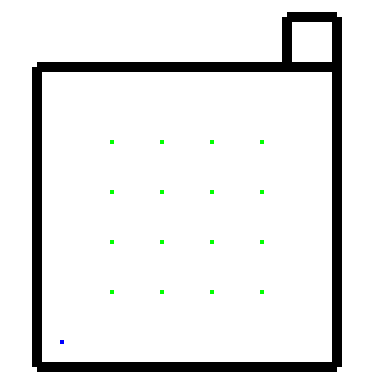
\includegraphics[scale=0.6]{figures/elderly_v1.png}
 \caption[知的エージェントの模式図]{知的エージェントの模式図 \label{elderly_v1}}
\end{center}
\end{figure}

\begin{figure}[htb]
\begin{center}
 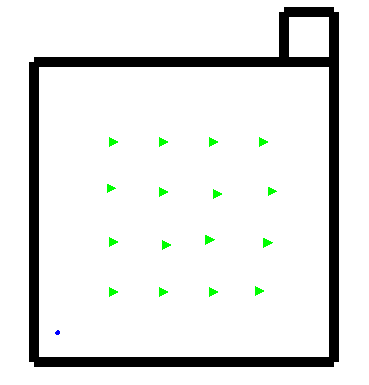
\includegraphics[scale=0.6]{figures/elderly_v2.png}
 \caption[知的エージェントの模式図]{知的エージェントの模式図 \label{elderly_v2}}
\end{center}
\end{figure}
% 2時間の中で排泄介助を行う
% 初期値として尿量を与える

\begin{figure}[htb]
\begin{center}
 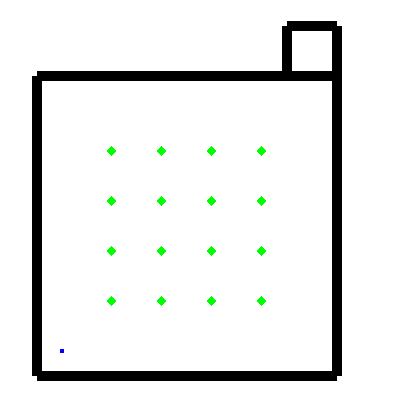
\includegraphics[scale=0.6]{figures/elderly_v3.png}
 \caption[知的エージェントの模式図]{知的エージェントの模式図 \label{elderly_v3}}
\end{center}
\end{figure}

\begin{figure}[htb]
\begin{center}
 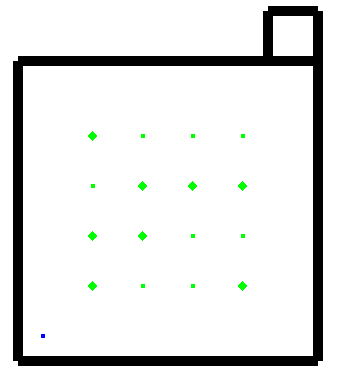
\includegraphics[scale=0.6]{figures/health_urinate.png}
 \caption[知的エージェントの模式図]{知的エージェントの模式図 \label{health_urinate}}
\end{center}
\end{figure}

\begin{figure}[htb]
\begin{center}
 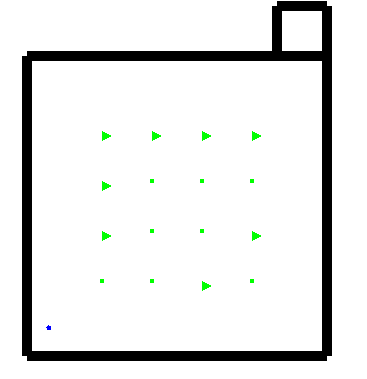
\includegraphics[scale=0.6]{figures/health_frequently_urinate_v1.png}
 \caption[知的エージェントの模式図]{知的エージェントの模式図 \label{health_frequently_urinate_v1}}
\end{center}
\end{figure}

\begin{figure}[htb]
\begin{center}
 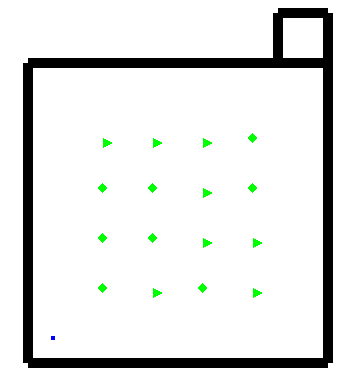
\includegraphics[scale=0.6]{figures/dementia_urinate_v1.png}
 \caption[知的エージェントの模式図]{知的エージェントの模式図 \label{dementia_urinate_v1}}
\end{center}
\end{figure}

\section{介護挙動の基本的な検証}

ATESの可視 化機 能を用いて交差 点における自動車と歩行者の相互作用の様子を可視化した とこ ろ,その相互作用が自然に行わ れている様 子を確 認できた,図11に は,そのスク リーンショットを小す.
% 人が1日に何回トイレに行くのかデータと実験値を比較させることによって,ある程度表現できていることを示したい.

\section{評価指標}

CaseVの目的は、CaseIの分断のない場合からCaselVの完全分 断への過程 (経緯)を解析すること に あ る。1(遮断率0%)とIV(遮断率100% ) を 除 き 中 間値を4段階 (遮断率20・40・60・80%)とし、その経緯を 占有率、平均搬送距離、変更過程、変 更回数、負傷者の 収 容・未 収 容 か ら検 討する。個々の医療 施設としてだけで はなく、分 断 過 程 に お け る 同一地域内の医療 施設 群とし ても評価 する。さ ら に、負傷者が 互いに競合して影響し合 う関係 を分析する こ と で総食 的に評価す る。占有率が早期段階で満床にな らない揚合に は平均搬送距離は長距離となるが、平均搬送 距離を短距離とする に は遠距離の負傷者を収容しない で早期毅階で満床と な る こ と が 必 要である。つま り、全体のバラン ス について考察する こ と も 必 要 で あ る。
% 合計我慢時間と成功回数で評価する.
% 十分な量に達していないときに介護を行なった場合は過剰介護,待たせてしまった場合はお漏らし処理などの追加業務が発生する.

\section{結果および考察}

図8に,車 両発生率・歩行者発 生率を そ れ ぞ れ変 化さ せ た場 合の シ ミュレーション結 果(lo回の試行の平均値 )を不 す.比較のた め に,飽和 交通流率の琿論値も示す,車両発生率が500台/時 間以.ヒで歩 行者発 生率が20人/サ イク ル以 上の場 合には,シ ミュレーション結 果と埋論 値の差は12% 以内で あり,両者は よく一致しているといえる,一方,車 両発生率が200台/時 間以 下の場 合,お よ び歩行 者発生率が5入/ サイ クルのときには,シ ミュレーション結果 が 理論値よ りもか なり低 くなっている.こ 居しは,これ らの条件で は道路 が飽和していないた めに発生する相 違であると考えられる.
